% "{'classe':('PSI'),'chapitre':'slci_correcteurs','type':('applications'),'titre':'Réglage de correcteurs P et PI', 'source':'P. Dupas','comp':('C1-02','C2-04'),'corrige':True}"
%\setchapterimage{bandeau}
\chapter*{Application \arabic{cptApplication} \\ 
Réglage de correcteurs P et PI -- 
\ifprof Corrigé \else Sujet \fi}
\addcontentsline{toc}{section}{Application \arabic{cptApplication} :
Réglage de correcteurs P et PI -- 
\ifprof Corrigé \else Sujet \fi}

\iflivret \stepcounter{cptApplication} \else
\ifprof  \stepcounter{cptApplication} \else \fi
\fi

\setcounter{question}{0}
\marginnote{Ressources de P. Dupas.}
%\marginnote[1cm]{
%\UPSTIcompetence[2]{C1-02}
%\UPSTIcompetence[2]{C2-04}}

\marginnote{\xpComp{COR}{02}\xpComp{COR}{03}}

%\begin{marginfigure} [4cm]
%\includegraphics[width=\linewidth]{fig_01a}
%\end{marginfigure}



%\subsection*{Correcteur proportionnel}
%Soit un système de fonction de transfert $G(p)=\dfrac{1}{\left(1+10p\right)\left(1+0,1p\right)\left(1+0,2p\right)}$ placé dans une boucle à retour unitaire.
%
%\question{Calculer la précision du système $\varepsilon_S$ pour une entrée échelon unitaire.}
%\ifprof
%\begin{corrige}
%Le système est de classe 0. L'entrée est de type échelon. $K_{\text{BO}}=1$.
%L'écart statique est de $\dfrac{1}{1+1}=\dfrac{1}{2}$.
%\end{corrige}
%\else
%\fi
%
%\question{Tracer dans  le diagramme de Bode la fonction de transfert en boucle ouverte du système.}
%\ifprof
%\begin{corrige}
%\begin{center}
%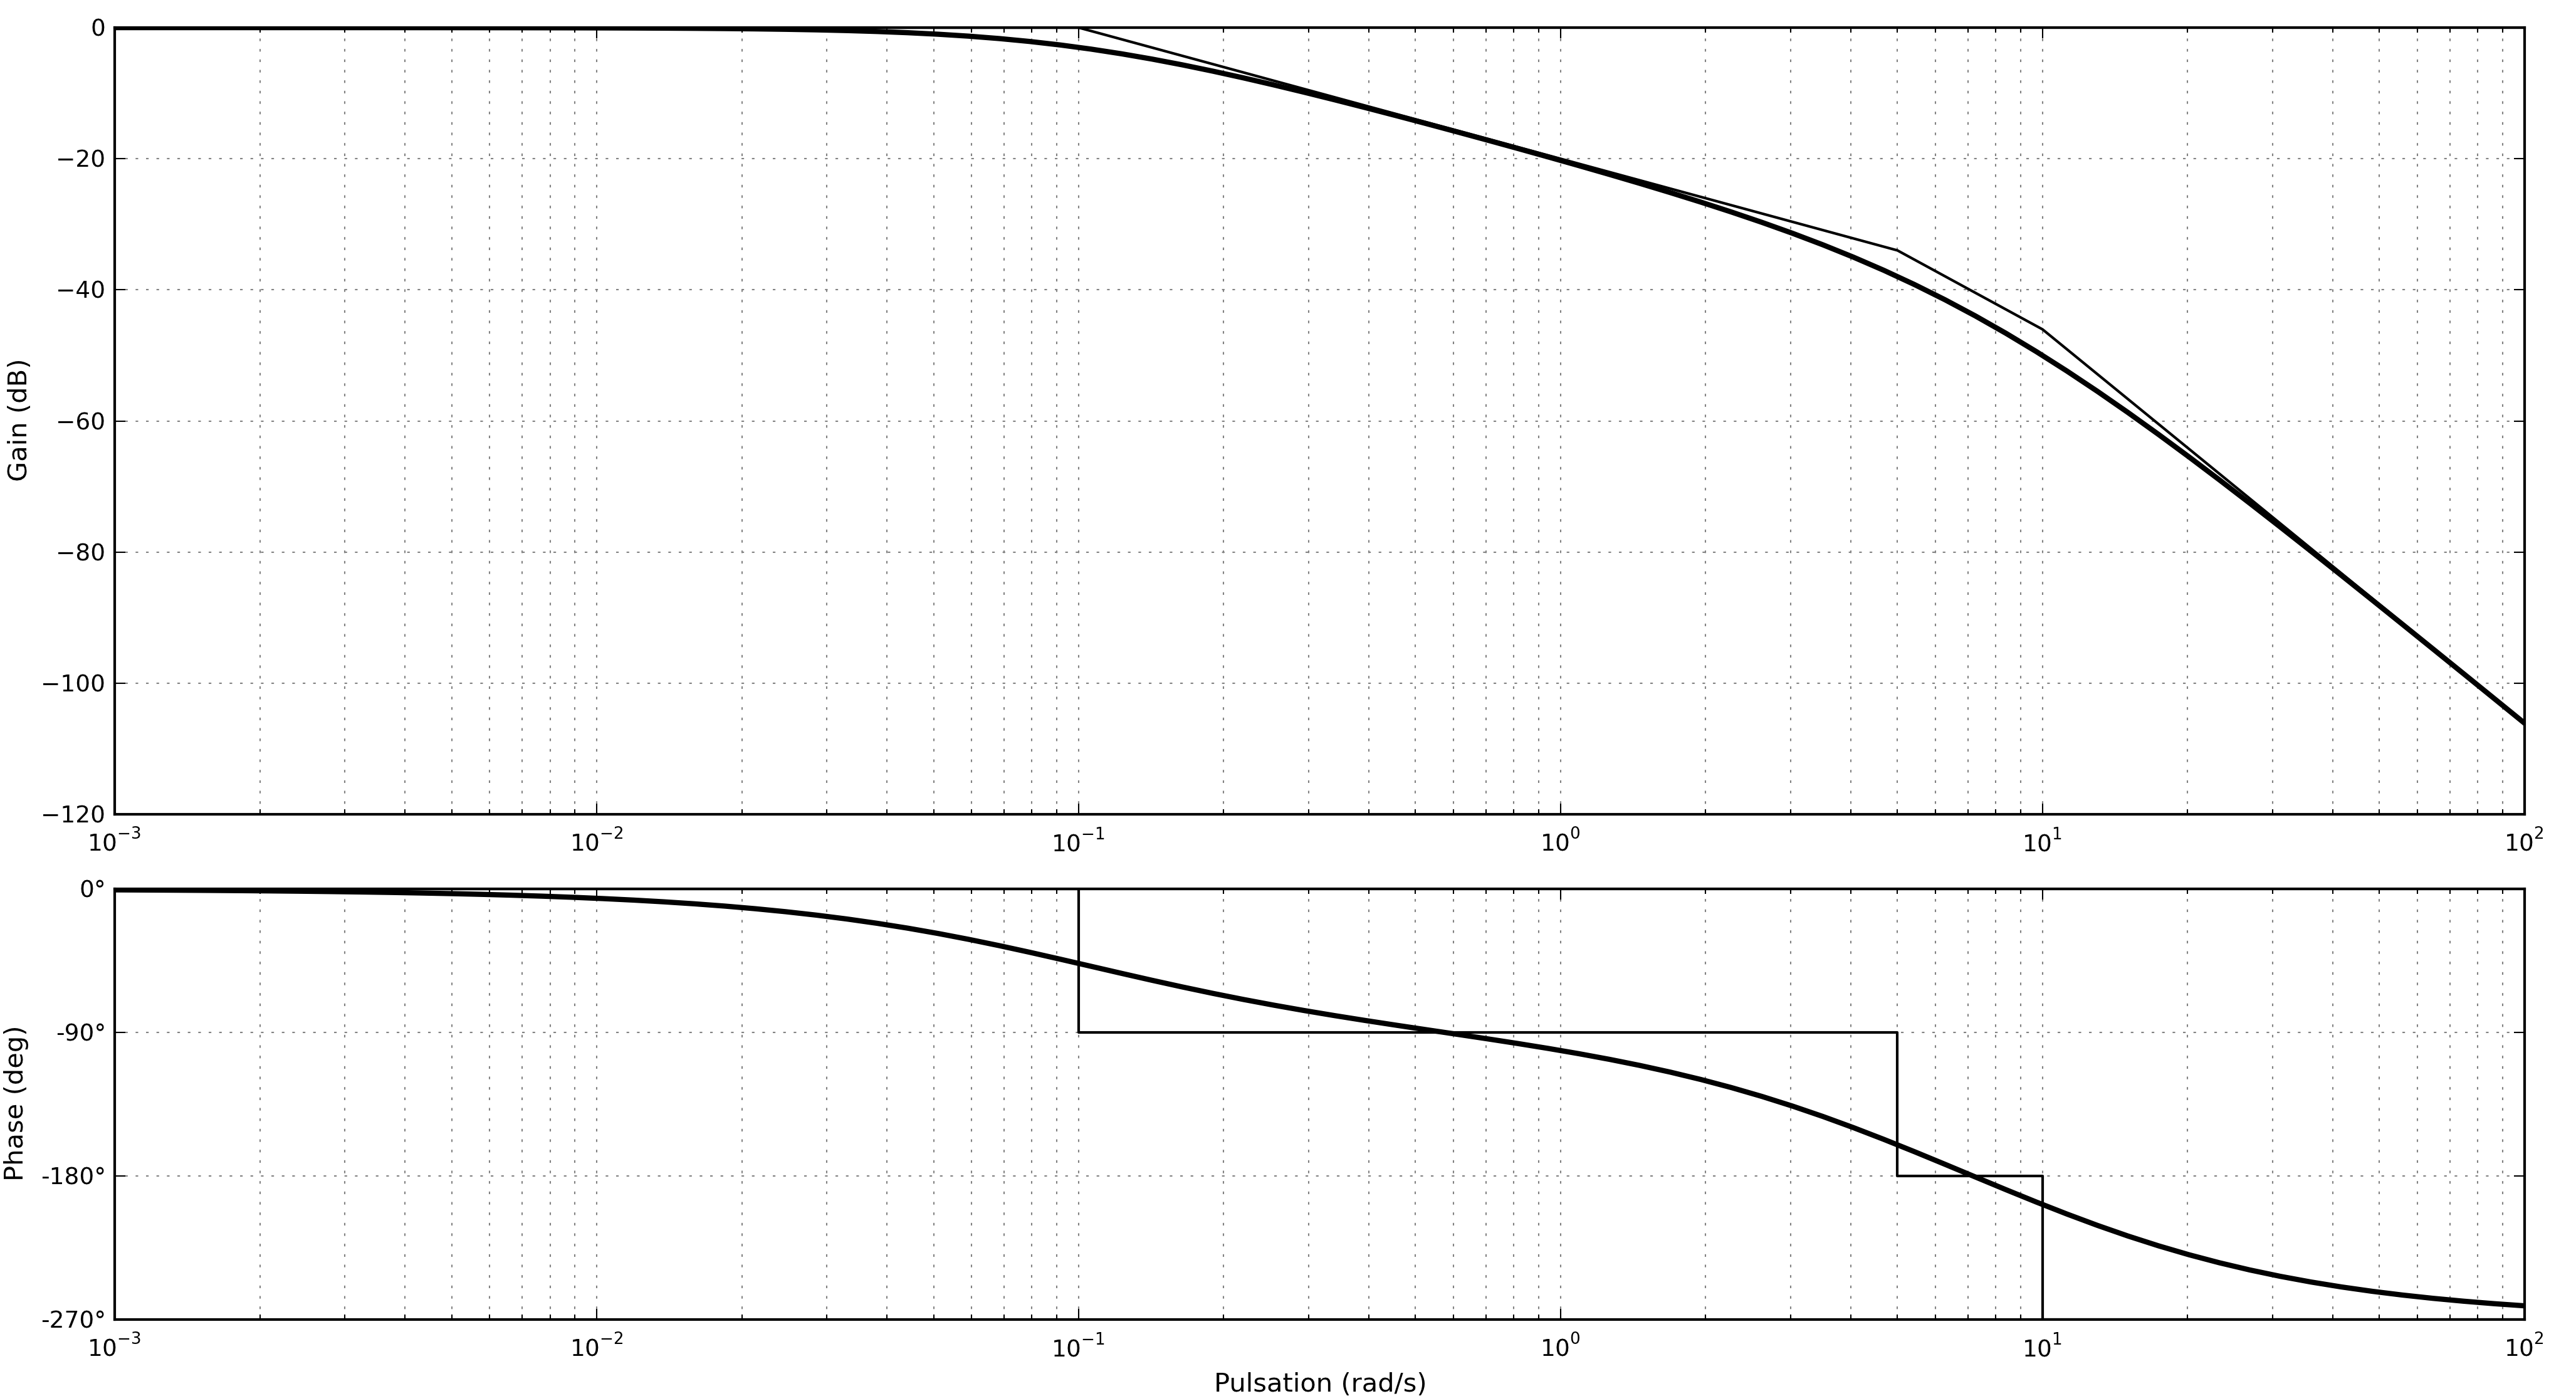
\includegraphics[width=.9\linewidth]{01_Bode}
%\end{center}
%\end{corrige}
%\else
%\fi
%
%
%\question{Déterminer $K$ pour avoir une marge de phase de 45\degres. Indiquer alors la valeur de la marge de gain. Indiquer la valeur de l'écart statique.}
%
%\ifprof
%\begin{corrige} ~\\
%
%\begin{itemize}
%\item On résout $\varphi\left(\omega\right)=-135\degres$ : 
%$\varphi\left(\omega\right)=-\arctan 10\omega-\arctan 0,1\omega-\arctan 0,2\omega$.
%
%$\varphi\left(\omega\right)=-135\degres \Leftrightarrow \omega = \SI{2,95}{rad.s^{-1}}$ (solveur Excel). 
%
%\item Calculons $G_{\text{dB}}(\omega)=-20\log\left(\sqrt{1+10^2\omega^2} \right)-20\log\left(\sqrt{1+0,1^2\omega^2} \right)-20\log\left(\sqrt{1+0,2^2\omega^2} \right)=\SI{-31}{dB}$. Il faut donc augmenter le gain de \SI{31}{dB} soit $K_P=10^{31/20}=35,48$.
%
%
%\item On a alors un écart statique de $\dfrac{1}{1+35,48}=0,027$.
%
%\item Pour déterminer la marge de gain, il faut résoudre $\varphi\left(\omega\right)=-180\degres$. On obtient $\omega=\SI{7,17}{rad/s}$ et $M_G=\SI{12}{dB}$.
%\end{itemize}
%
%
%\begin{center}
%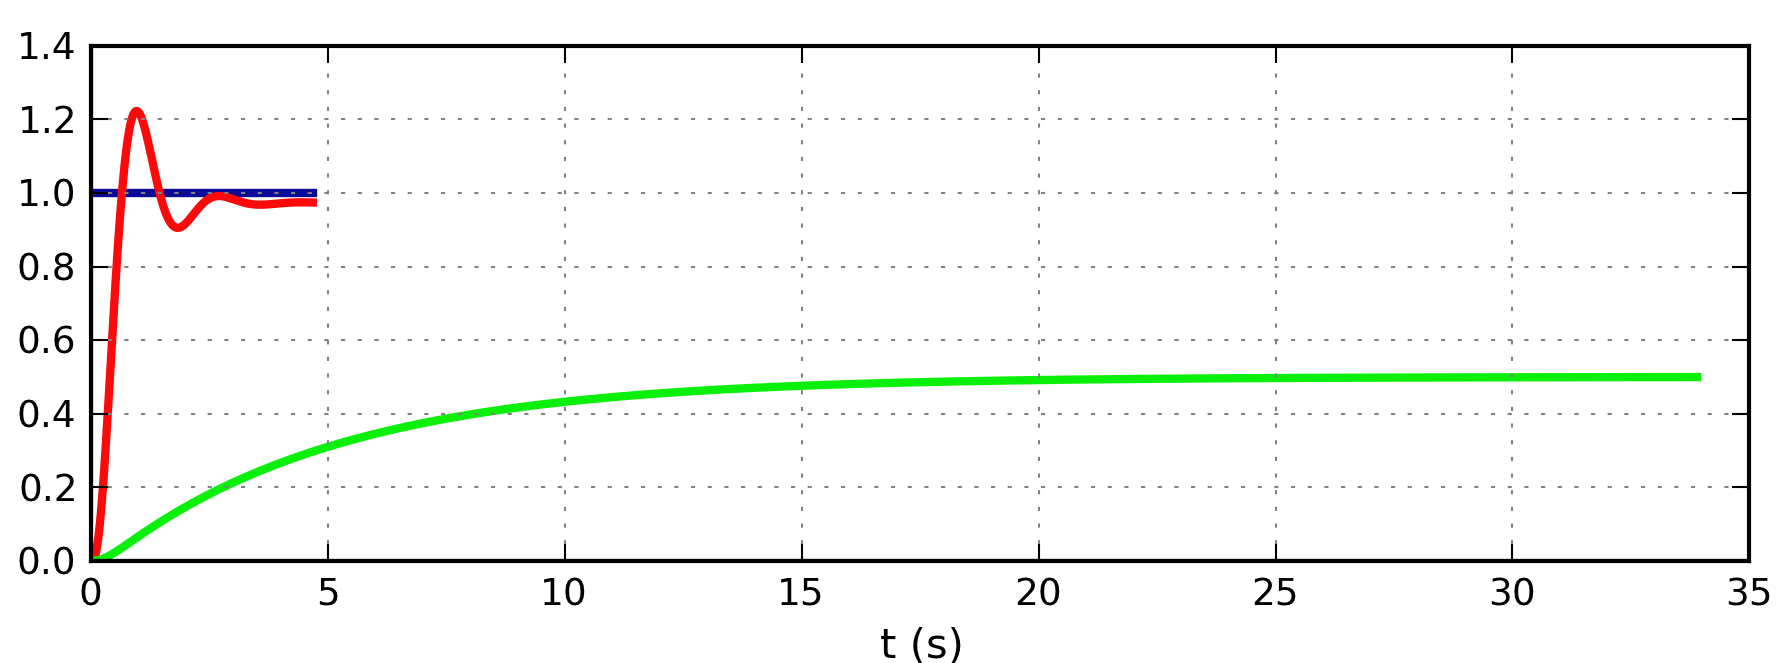
\includegraphics[width=.9\linewidth]{01_02}
%\end{center}
%
%\end{corrige}
%\else
%\fi
%
%
%\question{Déterminer $K$ pour avoir une marge de gain de \SI{6}{dB}. Indiquer alors la valeur de l'écart statique.}
%\ifprof
%\begin{corrige}
%\begin{itemize}
%\item On commence par résoudre $\varphi\left(\omega\right)=-180\degres$. On obtient $\omega=\SI{7,17}{rad/s}$ et $M_G=\SI{44}{dB}$.
%
%\item Il faut augmenter le gain de \SI{38}{dB} soit $20\log K_P=38\Rightarrow K_P=10^{38/20}=79$.
%
%
%\item On a alors un écart statique de $\dfrac{1}{1+79}=0,0125$.
%
%\item La marge de phase est alors de 19\degres. 
%\end{itemize}
%
%\begin{center}
%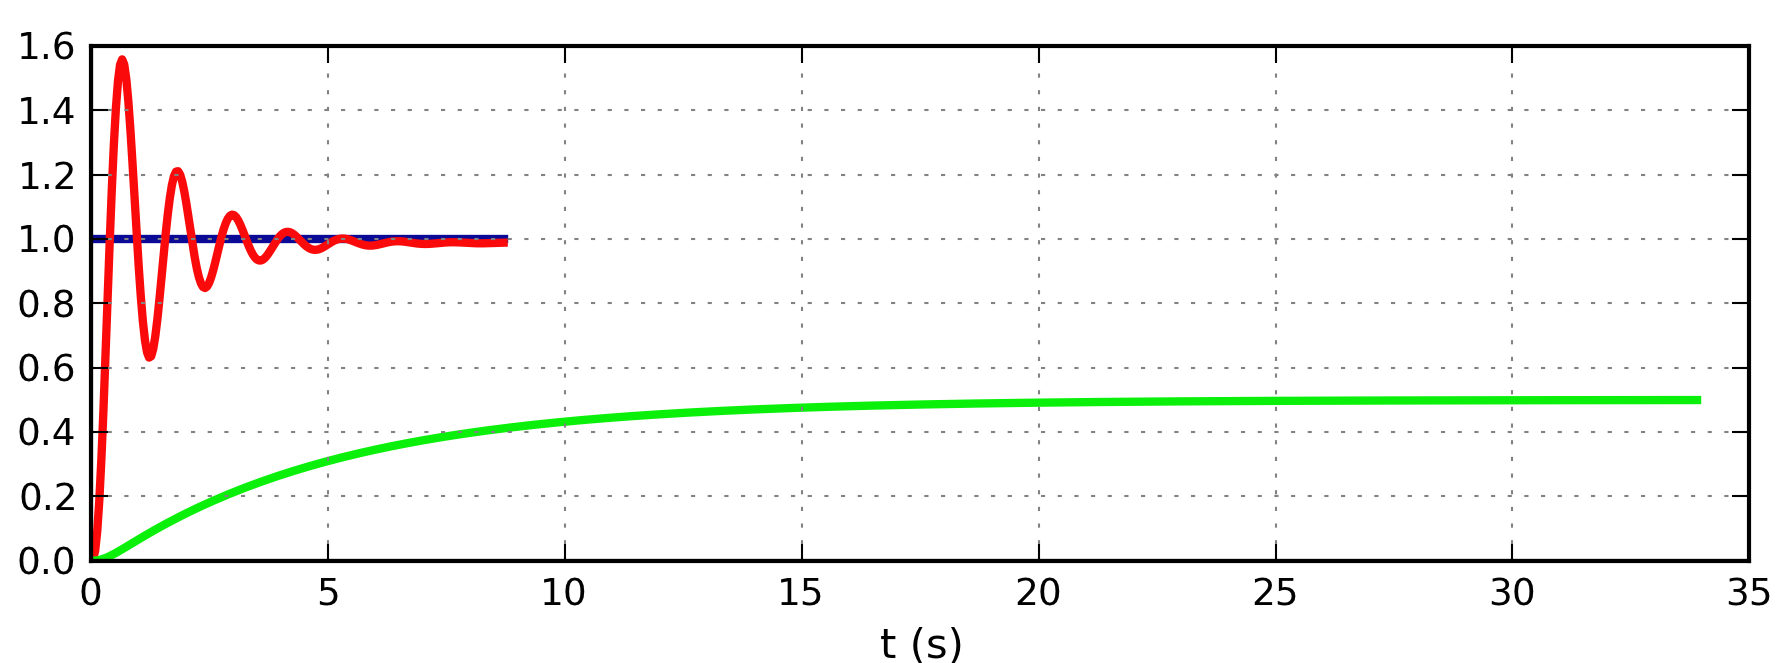
\includegraphics[width=.9\linewidth]{01_03}
%\end{center}
%
%\end{corrige}
%\else
%\fi
%
%
%\noindent
%\begin{tabular}{|p{.9\linewidth}|}
%\hline
%%\textit{Éléments de réponse}
%\begin{enumerate}
%\item $\varepsilon_S=\dfrac{1}{2}$.
%\item $\quad$.
%\item $\omega_{-135\degres}=\SI{2,95}{rad/s}$.
%\item $\omega_{\SI{0}{dB}}=\SI{7,17}{rad/s}$ et $M_G=\SI{38}{dB}$ soit $K_P=79$.
%\end{enumerate} \\
%\hline
%\end{tabular}
%\end{multicols}
%\ifprof
%\else
%\begin{center}
%\rotatebox{90}{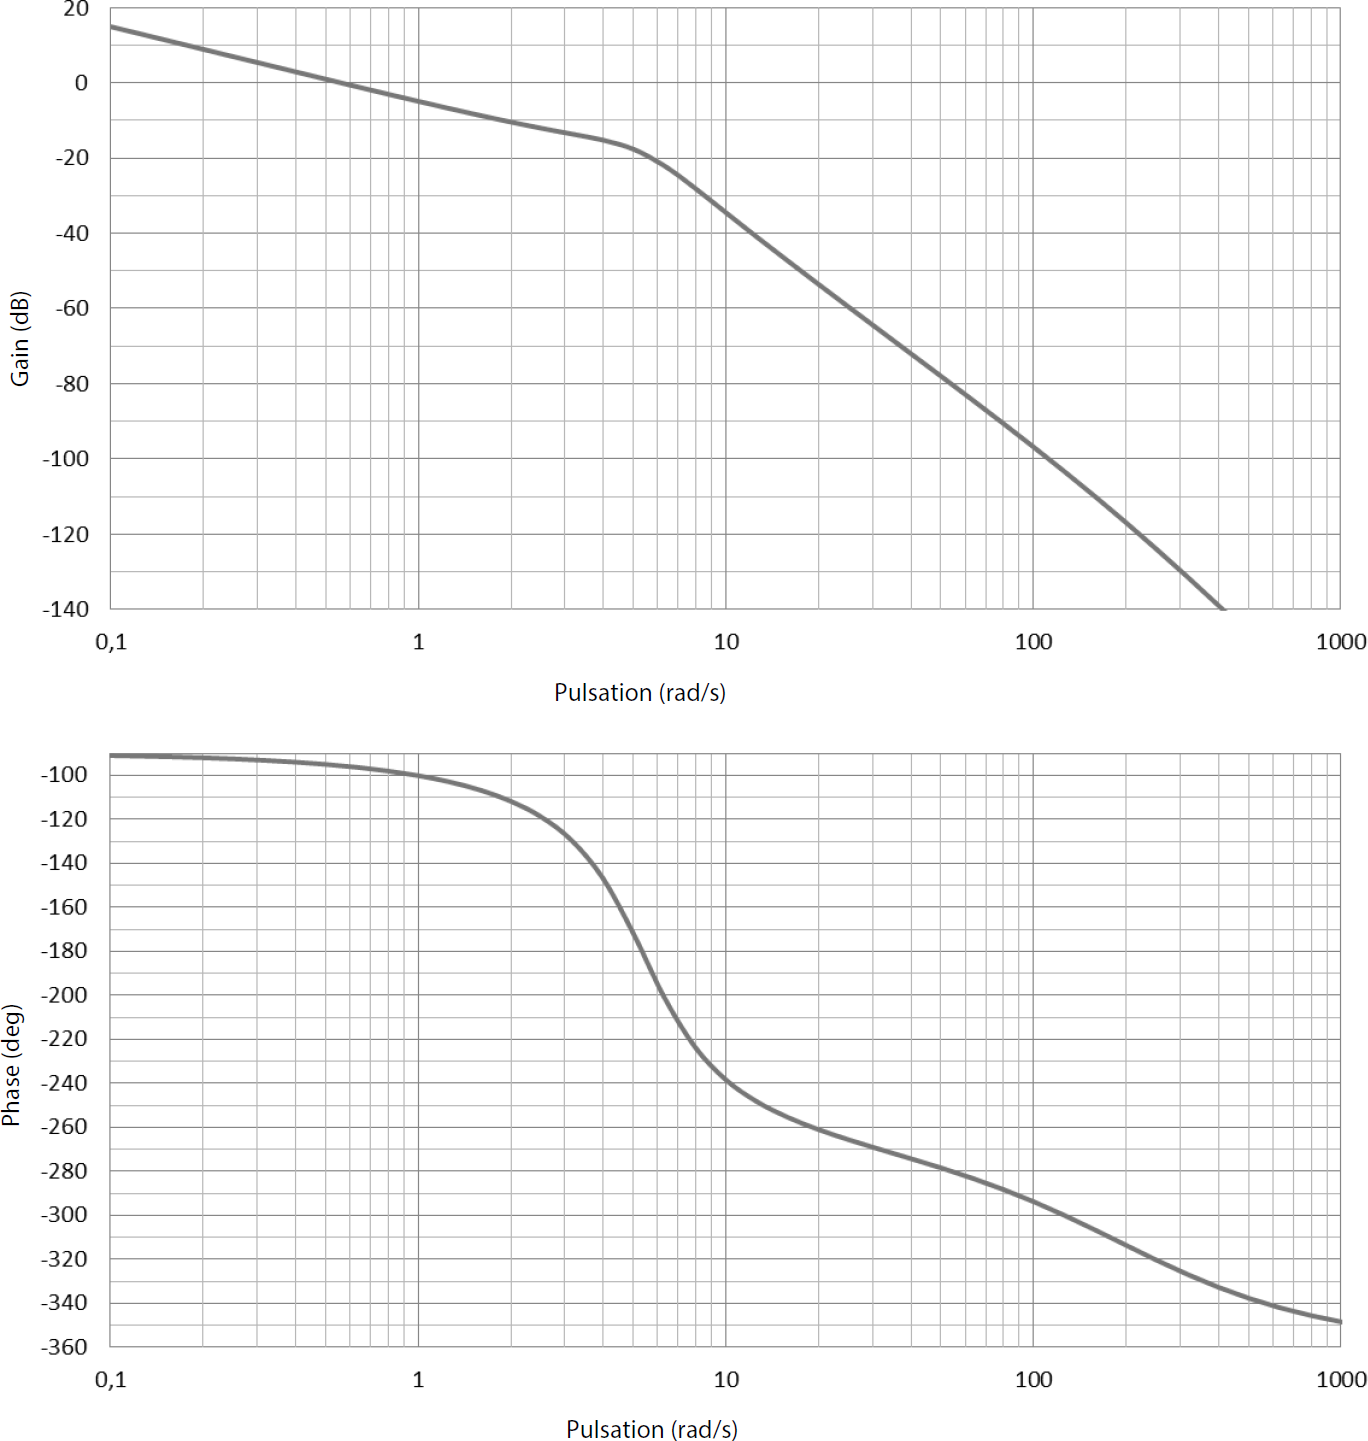
\includegraphics[width=.8\linewidth]{fig_04}}
%\end{center}
%
%\fi
%\begin{multicols}{2}
%
%
%\newpage
\subsection*{Correcteur proportionnel}
\marginnote{D'après ressources P. Dupas.}

\ifprof
\else
Soit un système de fonction de transfert $G(p)=\dfrac{10}{p\left(1+p+p^2\right)}$ placé dans une boucle à retour unitaire. On souhaite corriger le comportement de ce système par un correcteur proportionnel. On désire une marge de phase de \SI{45}{\degres} et une marge de gain de $\SI{10}{dB}$.

On donne le diagramme de Bode associé à cette fonction de transfert. 
\begin{center}
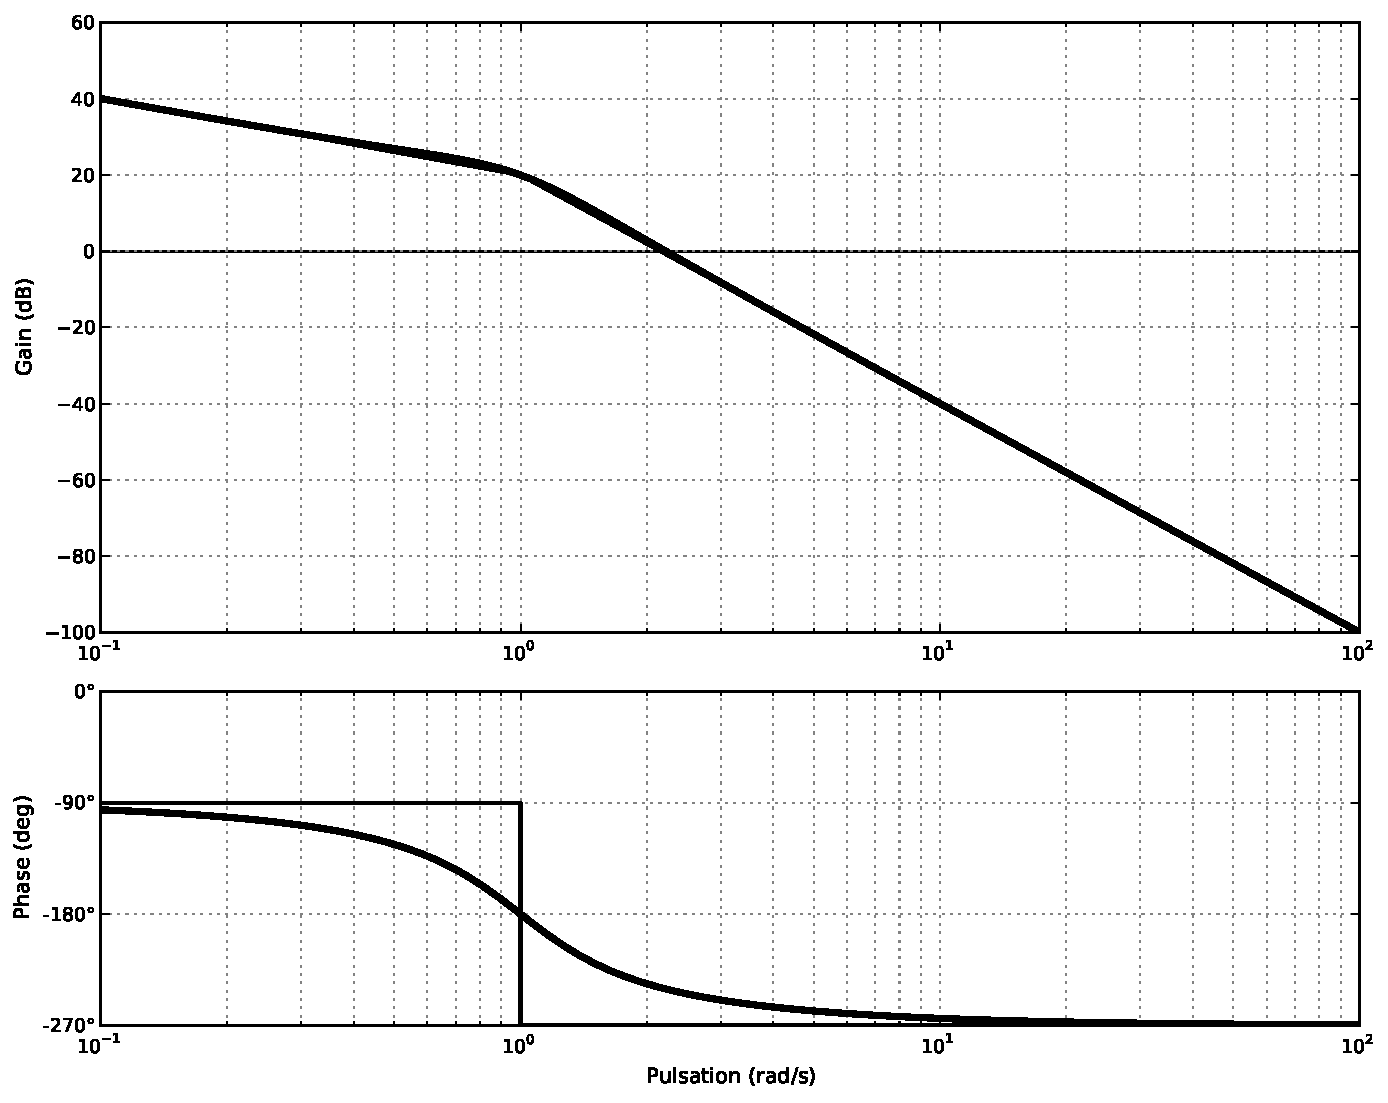
\includegraphics[width=\linewidth]{exo_01_bode}
\end{center}
\fi

\subsubsection*{Résolution graphique}



\question{Mesurer la marge de phase.}
\ifprof
\begin{corrige}~\\
\begin{itemize}
\item On cherche $\omega$ tel que $G_{\text{dB}}(\omega)=\SI{0}{dB}$  :
$G_{\text{dB}}(\omega)=-20\log(10) -20\log\omega-20\log\left(\sqrt{(1-\omega^2)^2+\omega^2}\right)$
\end{itemize}

On trouve $\omega=\SI{2,21}{rad/s}$ et $M_{\varphi}=-60\degres$. Le système est instable.
\end{corrige}
\else
\fi

\question{Mesurer la marge de gain.}
\ifprof
\begin{corrige}
Pour $\varphi=-180\degres$, on a $\omega=\SI{1}{rad/s}$ et $M_{G}=\SI{-20}{dB}$. Le système est instable.
\end{corrige}
\else
\fi

\question{Déterminer $K_p$ pour avoir une marge de phase de 45\degres. Vérifier la marge de gain.}
\ifprof
\begin{corrige}
Pour $\varphi=-135\degres$ on a $\omega=\SI{0,62}{rad/s}$. On trouve un gain proportionnel de 0,054.

La marge de gain est alors de \SI{5,35}{dB} ce qui est inférieur aux \SI{10}{dB} demandés.
\end{corrige}
\else
\fi

\question{Déterminer $K_p$ pour avoir une marge de gain de $\SI{10}{dB}$. Vérifier la marge de phase. }
\ifprof
\begin{corrige}
Pour $\varphi=-180\degres$ on a $\omega=\SI{1}{rad/s}$. On trouve un gain proportionnel de 0,316.

La marge de phase est alors de 70\degres ($\omega=\SI{0,0333}{rad/s})$.
\end{corrige}
\else
\fi

\subsubsection*{Résolution analytique}
\question{Calculer la marge de phase.}
\ifprof
\begin{corrige}~\\
\begin{itemize}
\item On cherche $\omega$ tel que $G_{\text{dB}}(\omega)=\SI{0}{dB}$  :
$G_{\text{dB}}(\omega)=-20\log(10) -20\log\omega-20\log\left(\sqrt{(1-\omega^2)^2+\omega^2}\right)$
\end{itemize}

On trouve $\omega=\SI{2,21}{rad/s}$ et $M_{\varphi}=-60\degres$. Le système est instable.
\end{corrige}
\else
\fi

\question{Calculer la marge de gain.}
\ifprof
\begin{corrige}
Pour $\varphi=-180\degres$, on a $\omega=\SI{1}{rad/s}$ et $M_{G}=\SI{-20}{dB}$. Le système est instable.
\end{corrige}
\else
\fi

\question{Calculer $K_p$ pour avoir une marge de phase de 45\degres. Vérifier la marge de gain. }
\ifprof
\begin{corrige}
Pour $\varphi=-135\degres$ on a $\omega=\SI{0,62}{rad/s}$. On trouve un gain proportionnel de 0,054.

La marge de gain est alors de \SI{5,35}{dB} ce qui est inférieur aux \SI{10}{dB} demandés.
\end{corrige}
\else
\fi

\question{Calculer $K_p$ pour avoir une marge de gain de $\SI{10}{dB}$. Vérifier la marge de phase. }
\ifprof
\begin{corrige}
Pour $\varphi=-180\degres$ on a $\omega=\SI{1}{rad/s}$. On trouve un gain proportionnel de 0,316.

La marge de phase est alors de 70\degres ($\omega=\SI{0,0333}{rad/s})$.
\end{corrige}
\else
\fi


\ifcolle
\else
\ifprof 
\else
\marginnote{
\begin{solution}
\begin{enumerate}
\item $M_{\varphi}=-60\degres$.
\item $M_G=\SI{-20}{dB}$.
\item $K_P=0,054$ et $M_{G}=\SI{5,35}{dB}$.
\item $K_P=0,0316$ et $M_{\varphi}=70\degres$.
\end{enumerate}
\end{solution}}
\fi
\fi

%\subsection*{Correcteur proportionnel} % TETE DE LECTURE
%Soit un système de fonction de transfert $G(p)=\dfrac{1}{\left(1+0,05p\right)\left(1+p+2p^2\right)}$. On souhaite corriger le comportement de ce système par un correcteur proportionnel.
%\subparagraph*{}\textit{Déterminer le gain $K$ qui assure une marge de phase de 45\degres.}
%
%
%\subsection*{Correcteur proportionnel}

\subsection*{Correcteur proportionnel intégral}
\marginnote{D'après ressources P. Dupas.}

\ifprof
\else
Soit un système de fonction de transfert $G(p)=\dfrac{1}{\left(p+1\right)\left(\dfrac{p}{8}+1\right)}$ placé dans une boucle à retour unitaire.

On souhaite disposer d'une marge de phase de 45\degres en utilisant un correcteur proportionnel intégral de la forme $C(p)=K_p\dfrac{1+\tau p}{\tau p}$.
\fi

\question[Falcultatif]{Justifier le diagramme de Bode de la boucle ouverte non corrigée.}
\ifprof
\begin{corrige}
\begin{center}
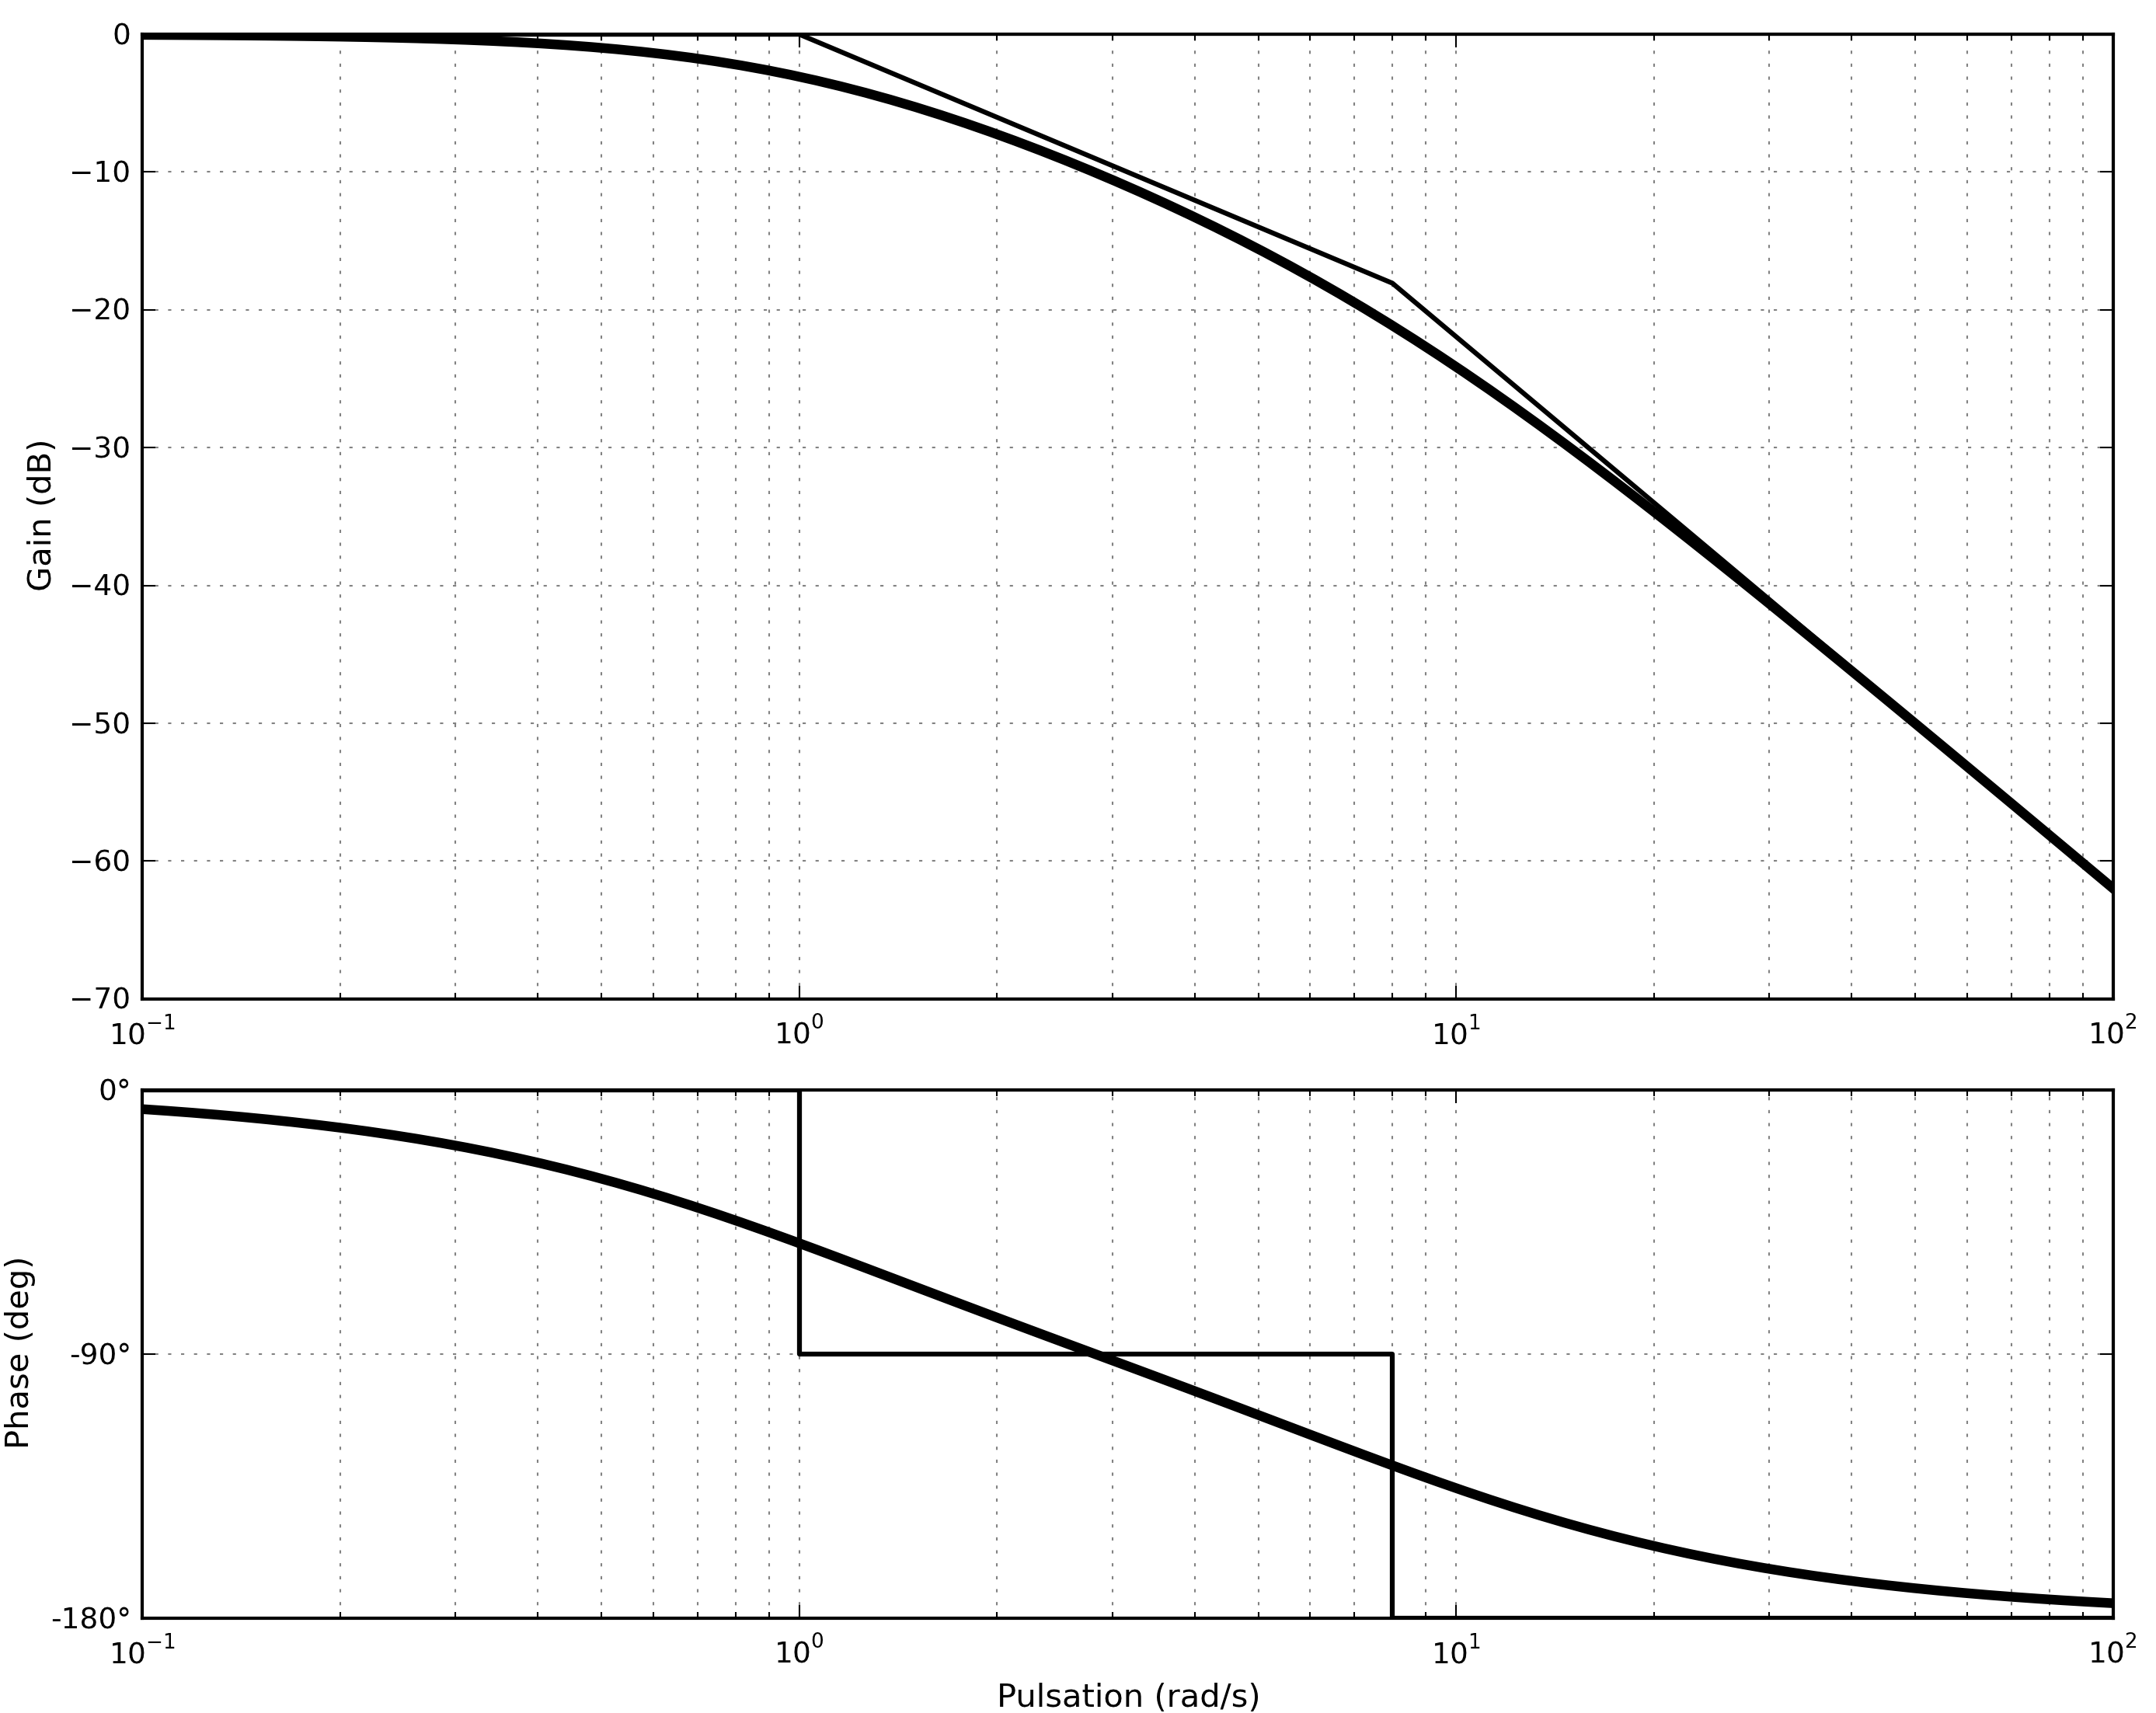
\includegraphics[width=\linewidth]{PI_BodeNC}
\end{center}
\end{corrige}
\else
\begin{center}
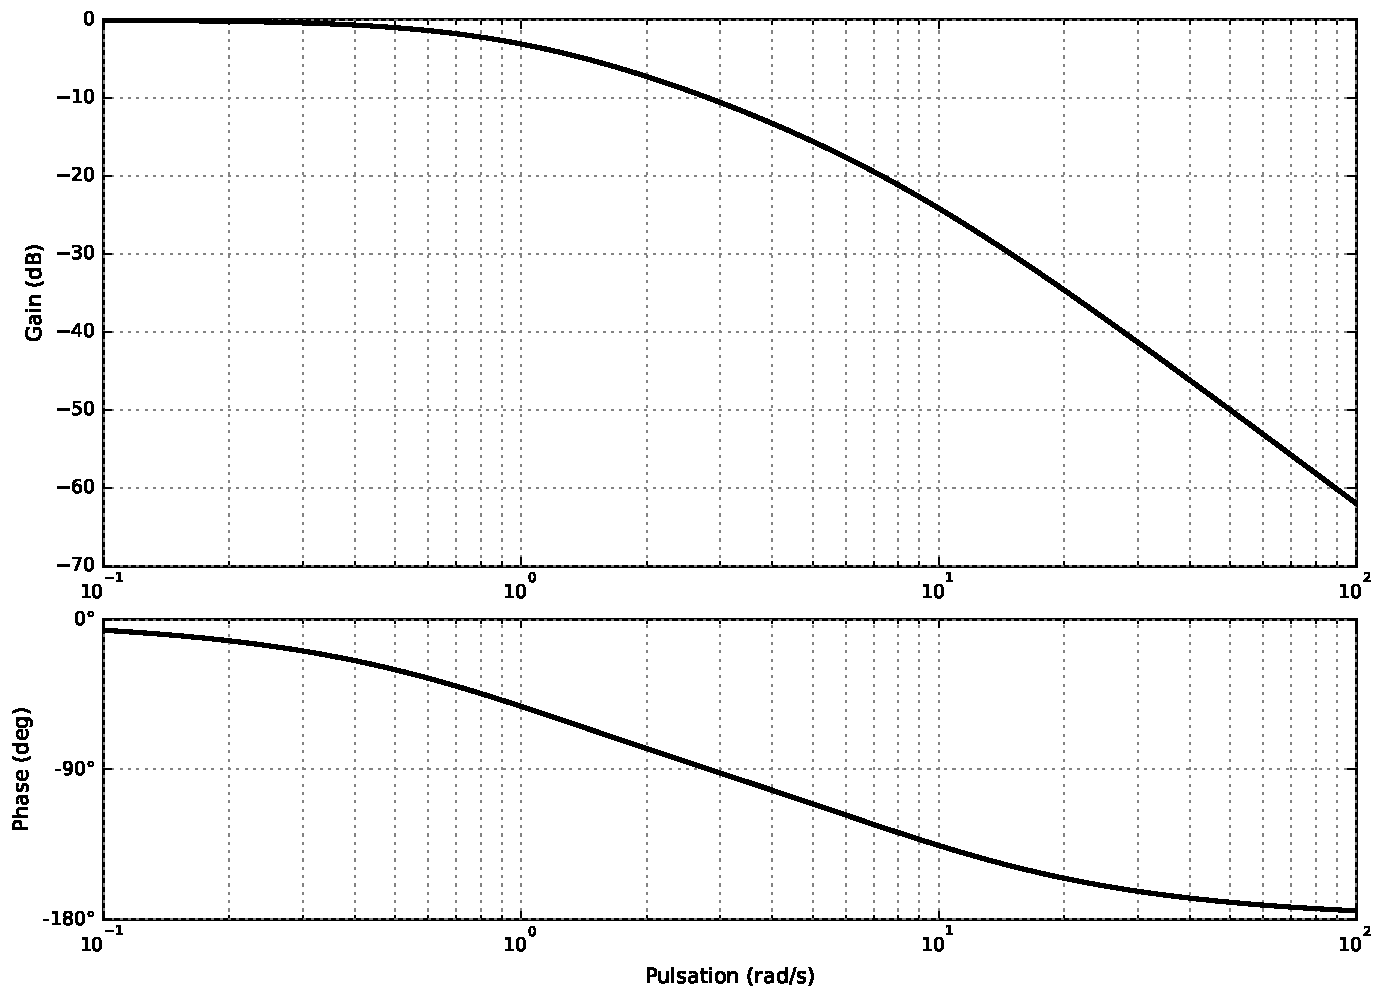
\includegraphics[width=\linewidth]{exo_02_bode}
\end{center}
\fi


\question{Déterminer graphiquement les paramètres du correcteur pour avoir une marge de phase de 45\degres. }

\question{Déterminer analytiquement les paramètres du correcteur pour avoir une marge de phase de 45\degres. }
\ifprof
\begin{corrige}~\\

\begin{itemize}
\item On résout $\varphi\left(\omega\right)=-135\degres$ : 
$\varphi\left(\omega\right)=-\arctan \omega-\arctan \omega/8 $ $\Rightarrow \tan 135\degres = \dfrac{\omega+\omega/8}{1-\omega^2/8}$ 
$\Leftrightarrow - 1+\omega^2/8-9\omega/8=0$ 
$\Leftrightarrow  \omega^2 -9\omega-8 =0$. 
$\Delta = 81+32=10,63^2$. 
$\omega = \dfrac{9\pm10,63}{2}=\SI{9,82}{rad/s}$.


\item Calculons $G_{\text{dB}}(9,82)=\SI{-23,9}{dB}$. Il faut donc augmenter le gain de \SI{23,9}{dB} soit $K_P=10^{23,9/20}=15,7$.

\item On choisit $\tau$ pour ne pas modifier la marge de phase. Il faut donc que le déphasage de 0\degres du correcteur ait lieu  avant \SI{9,82}{rad/s}. De manière usuelle on prend $\dfrac{1}{\tau}=\dfrac{9,82}{10}=\SI{0,982}{rad/s}$.

\item Au final, on a $C(p)=15,7\dfrac{1+1,018p}{1,018p}$.
\end{itemize}

\end{corrige}
\else\fi

\question{Tracer le diagramme de Bode du correcteur et le diagramme de la boucle ouverte corrigée.}

\ifprof
\begin{corrige}~\\
\begin{center}
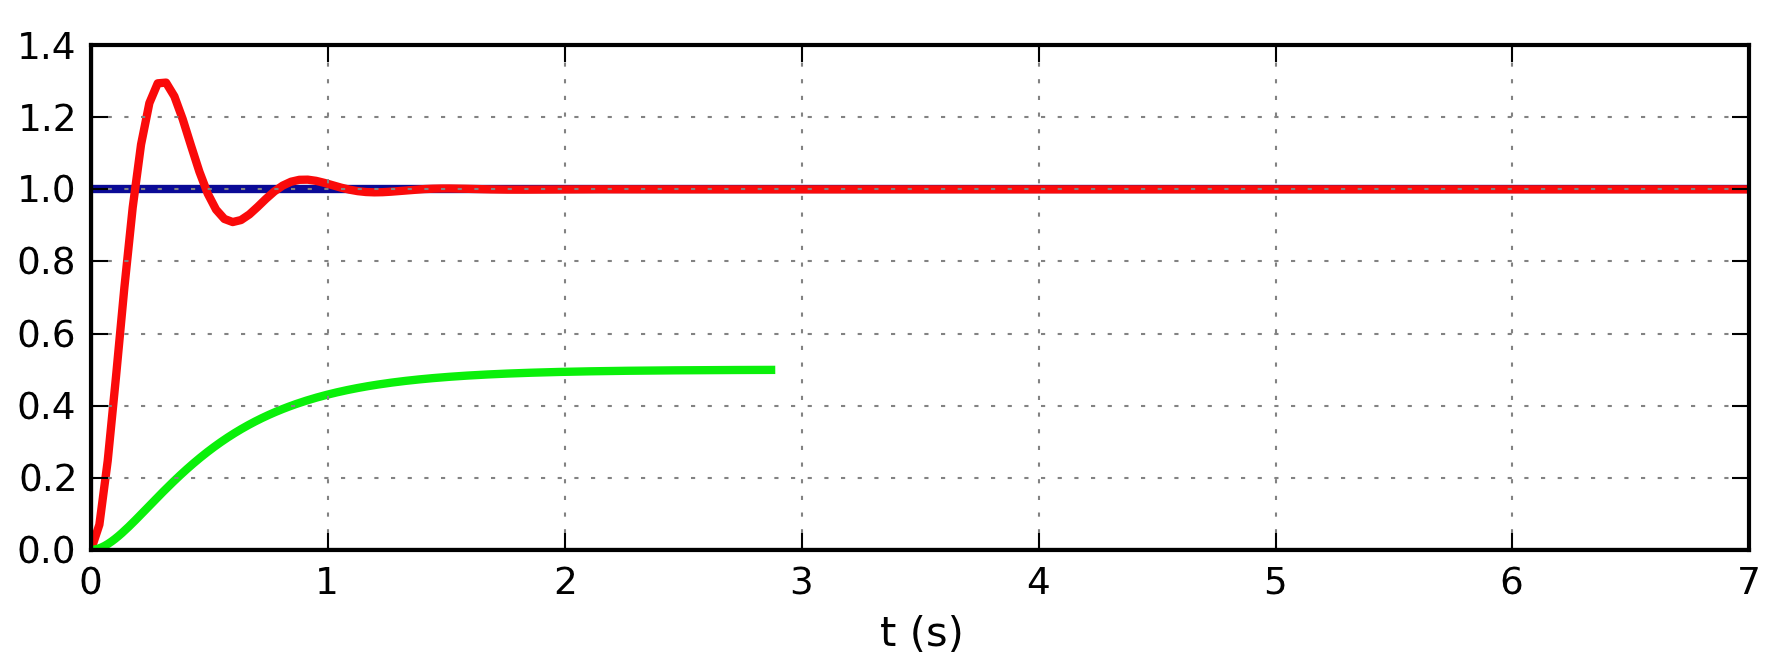
\includegraphics[width=\linewidth]{PI_corrige.png}
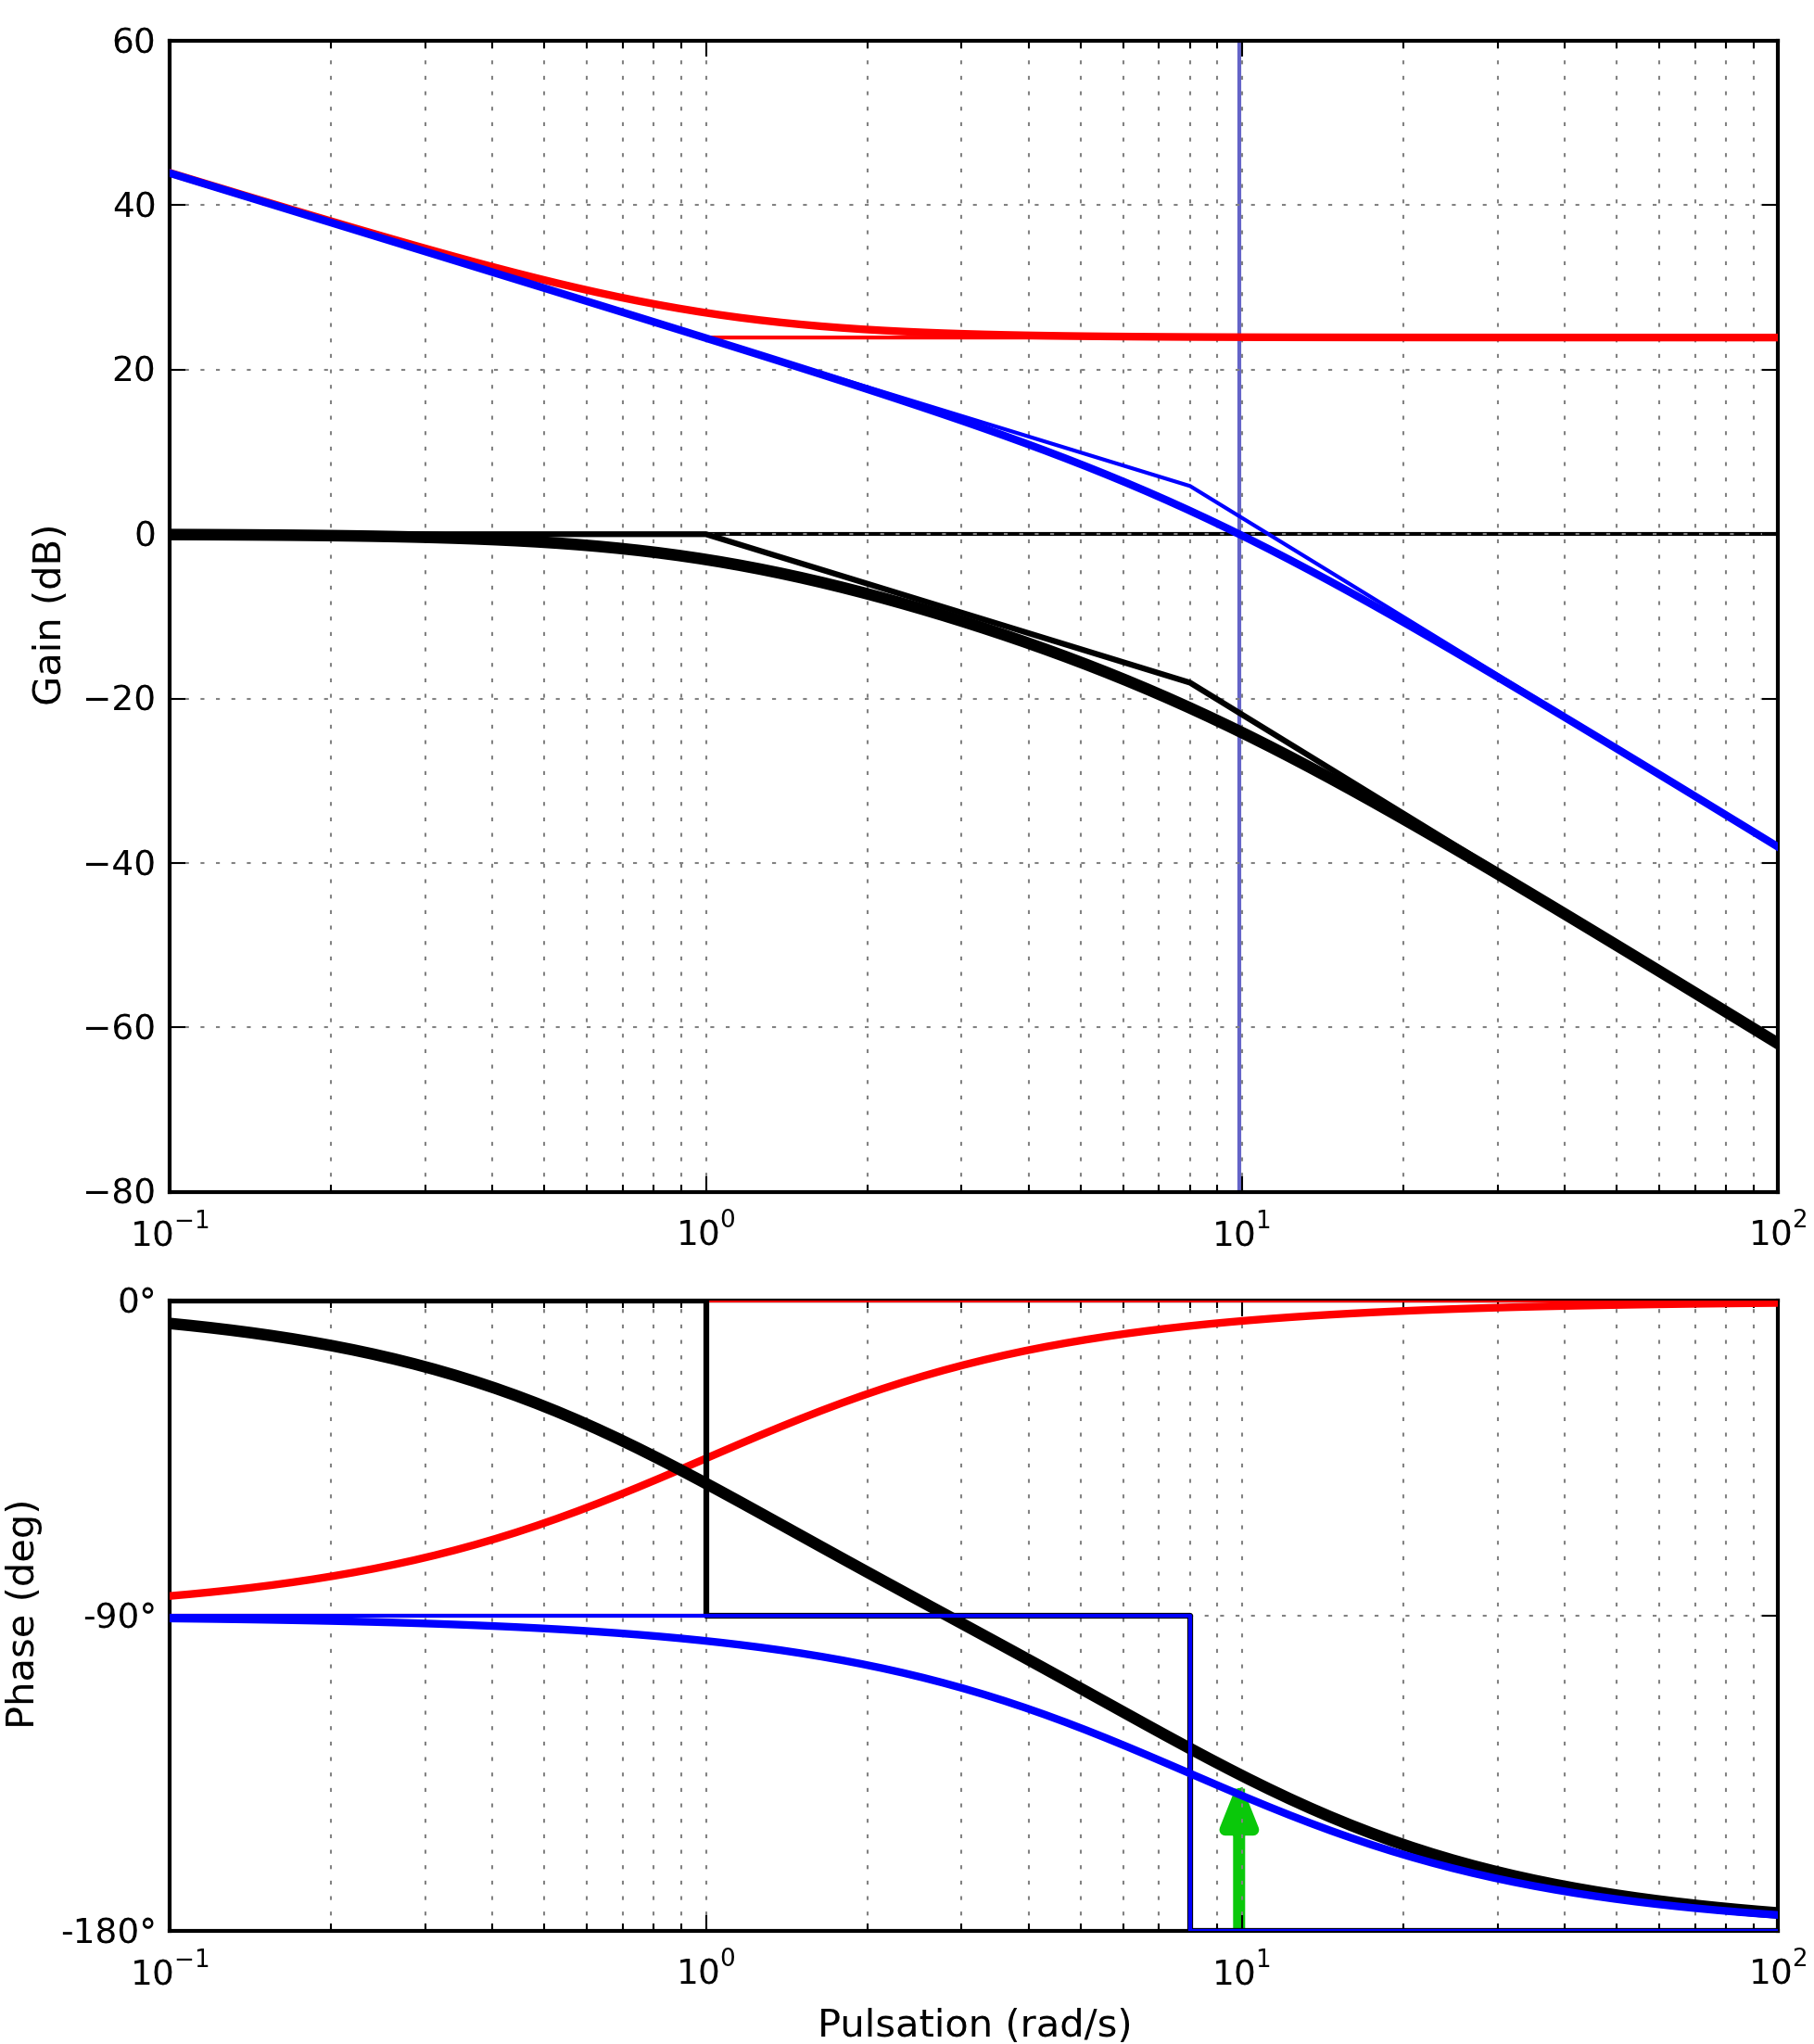
\includegraphics[width=\linewidth]{PI_BodeC.png}
\end{center}
\end{corrige}
\else
\fi


\ifprof
\else
\begin{marginfigure}
\centering

\includegraphics[width=3cm]{Cy_03_01_Activation_01_P_PI_qr}
\end{marginfigure}
\fi


\ifcolle
\else
\ifprof
\else
\marginnote{
\begin{solution}
\begin{enumerate}
\item $\quad$
\item $C(p)=15,7\dfrac{1+1,018p}{1,018p}$.
\item $\quad$
\end{enumerate}
\end{solution}}
\fi
\fi

%\end{multicols}

%
%
%\subsection*{Correcteur à avance de phase}
%\setcounter{exo}{0}
%Soit un système de fonction de transfert $G(p)=\dfrac{100}{\left(p+1\right)^2}$ placé dans une boucle à retour unitaire. On souhaite corrige ce système en utilisant un correcteur à avance de phase de la forme $C(p)=K\dfrac{1+a\tau p}{1+\tau p}$.
%
%
%\question{Tracer le diagramme de Bode de $G(p)$.}
%
%
%\question{Corriger ce système de sorte que sa marge de phase soit égale à 45\degres.}
%\ifprof
%\begin{corrige}~\\
%\begin{itemize}
%\item $G_{\text{dB}}(\omega)=20\log \left(100\right)-20\log\left(1+\omega^2\right)$. $G_{\text{dB}}(\omega)=0 \Leftrightarrow \dfrac{100}{1+\omega^2}=1$ $  \Leftrightarrow \omega=\pm\sqrt{99}$ $\Rightarrow \omega=\SI{9,95}{rad/s}$.
%\item $\varphi(\omega)=-2\arctan\omega$ et $\varphi(9,95)=-\SI{2,94}{rad}=-169\degres$ soit une marge de phase de 11\degres; le correcteur doit donc apporter un complément de phase de 34\degres. 
%\item $\varphi_{\text{max}}=\arcsin\left( \dfrac{a-1}{a+1}\right)\Rightarrow \sin \left(\varphi_{\text{max}}\right)=\dfrac{a-1}{a+1}$ 
%$\Rightarrow a=-\dfrac{\sin \left(\varphi_{\text{max}}\right)+1}{ \sin \left(\varphi_{\text{max}}\right) -1}=3,54$.
%\item $\tau=\dfrac{1}{9,95\sqrt{3,54}}=\SI{0,053}{s}$.
%\end{itemize}
%\end{corrige}
%%\ifprof
%%\begin{itemize}
%%\item Pulsation de coupure à \SI{0}{dB} su système non corrigé en BO : $\omega=\SI{9,95}{rad.s^{-1}}$.
%%\item Pour cette pulsation la marge de phase est de 11\degres.
%%\item On cherche $\varphi_{\text{max}}=25\degres$ et $a=3,54$. 
%%\item $\omega_{\text{max}}=\SI{9,95}{rad.s^{-1}}= \dfrac{1}{T\sqrt{a}}$ %ce qui conduit à $T=\SI{0,053}{s}$.
%%\item $K=\dfrac{1}{\sqrt{a}}=0,53$.
%%\end{itemize}
%\else
%\fi
%
%
%\question{Tracer le diagramme de Bode du correcteur et le diagramme de la boucle ouverte corrigée.}
%
%\noindent
%\begin{tabular}{|p{.9\linewidth}|}
%\hline
%\begin{enumerate}
%\item $\quad$
%\item $C(p)=0,53\dfrac{1+3,54 \cdot 0,053  p}{1+0,053 p}$.
%\item $\quad$
%\end{enumerate}\\
%\hline
%\end{tabular}

%
%\ifprof
%\begin{center}
%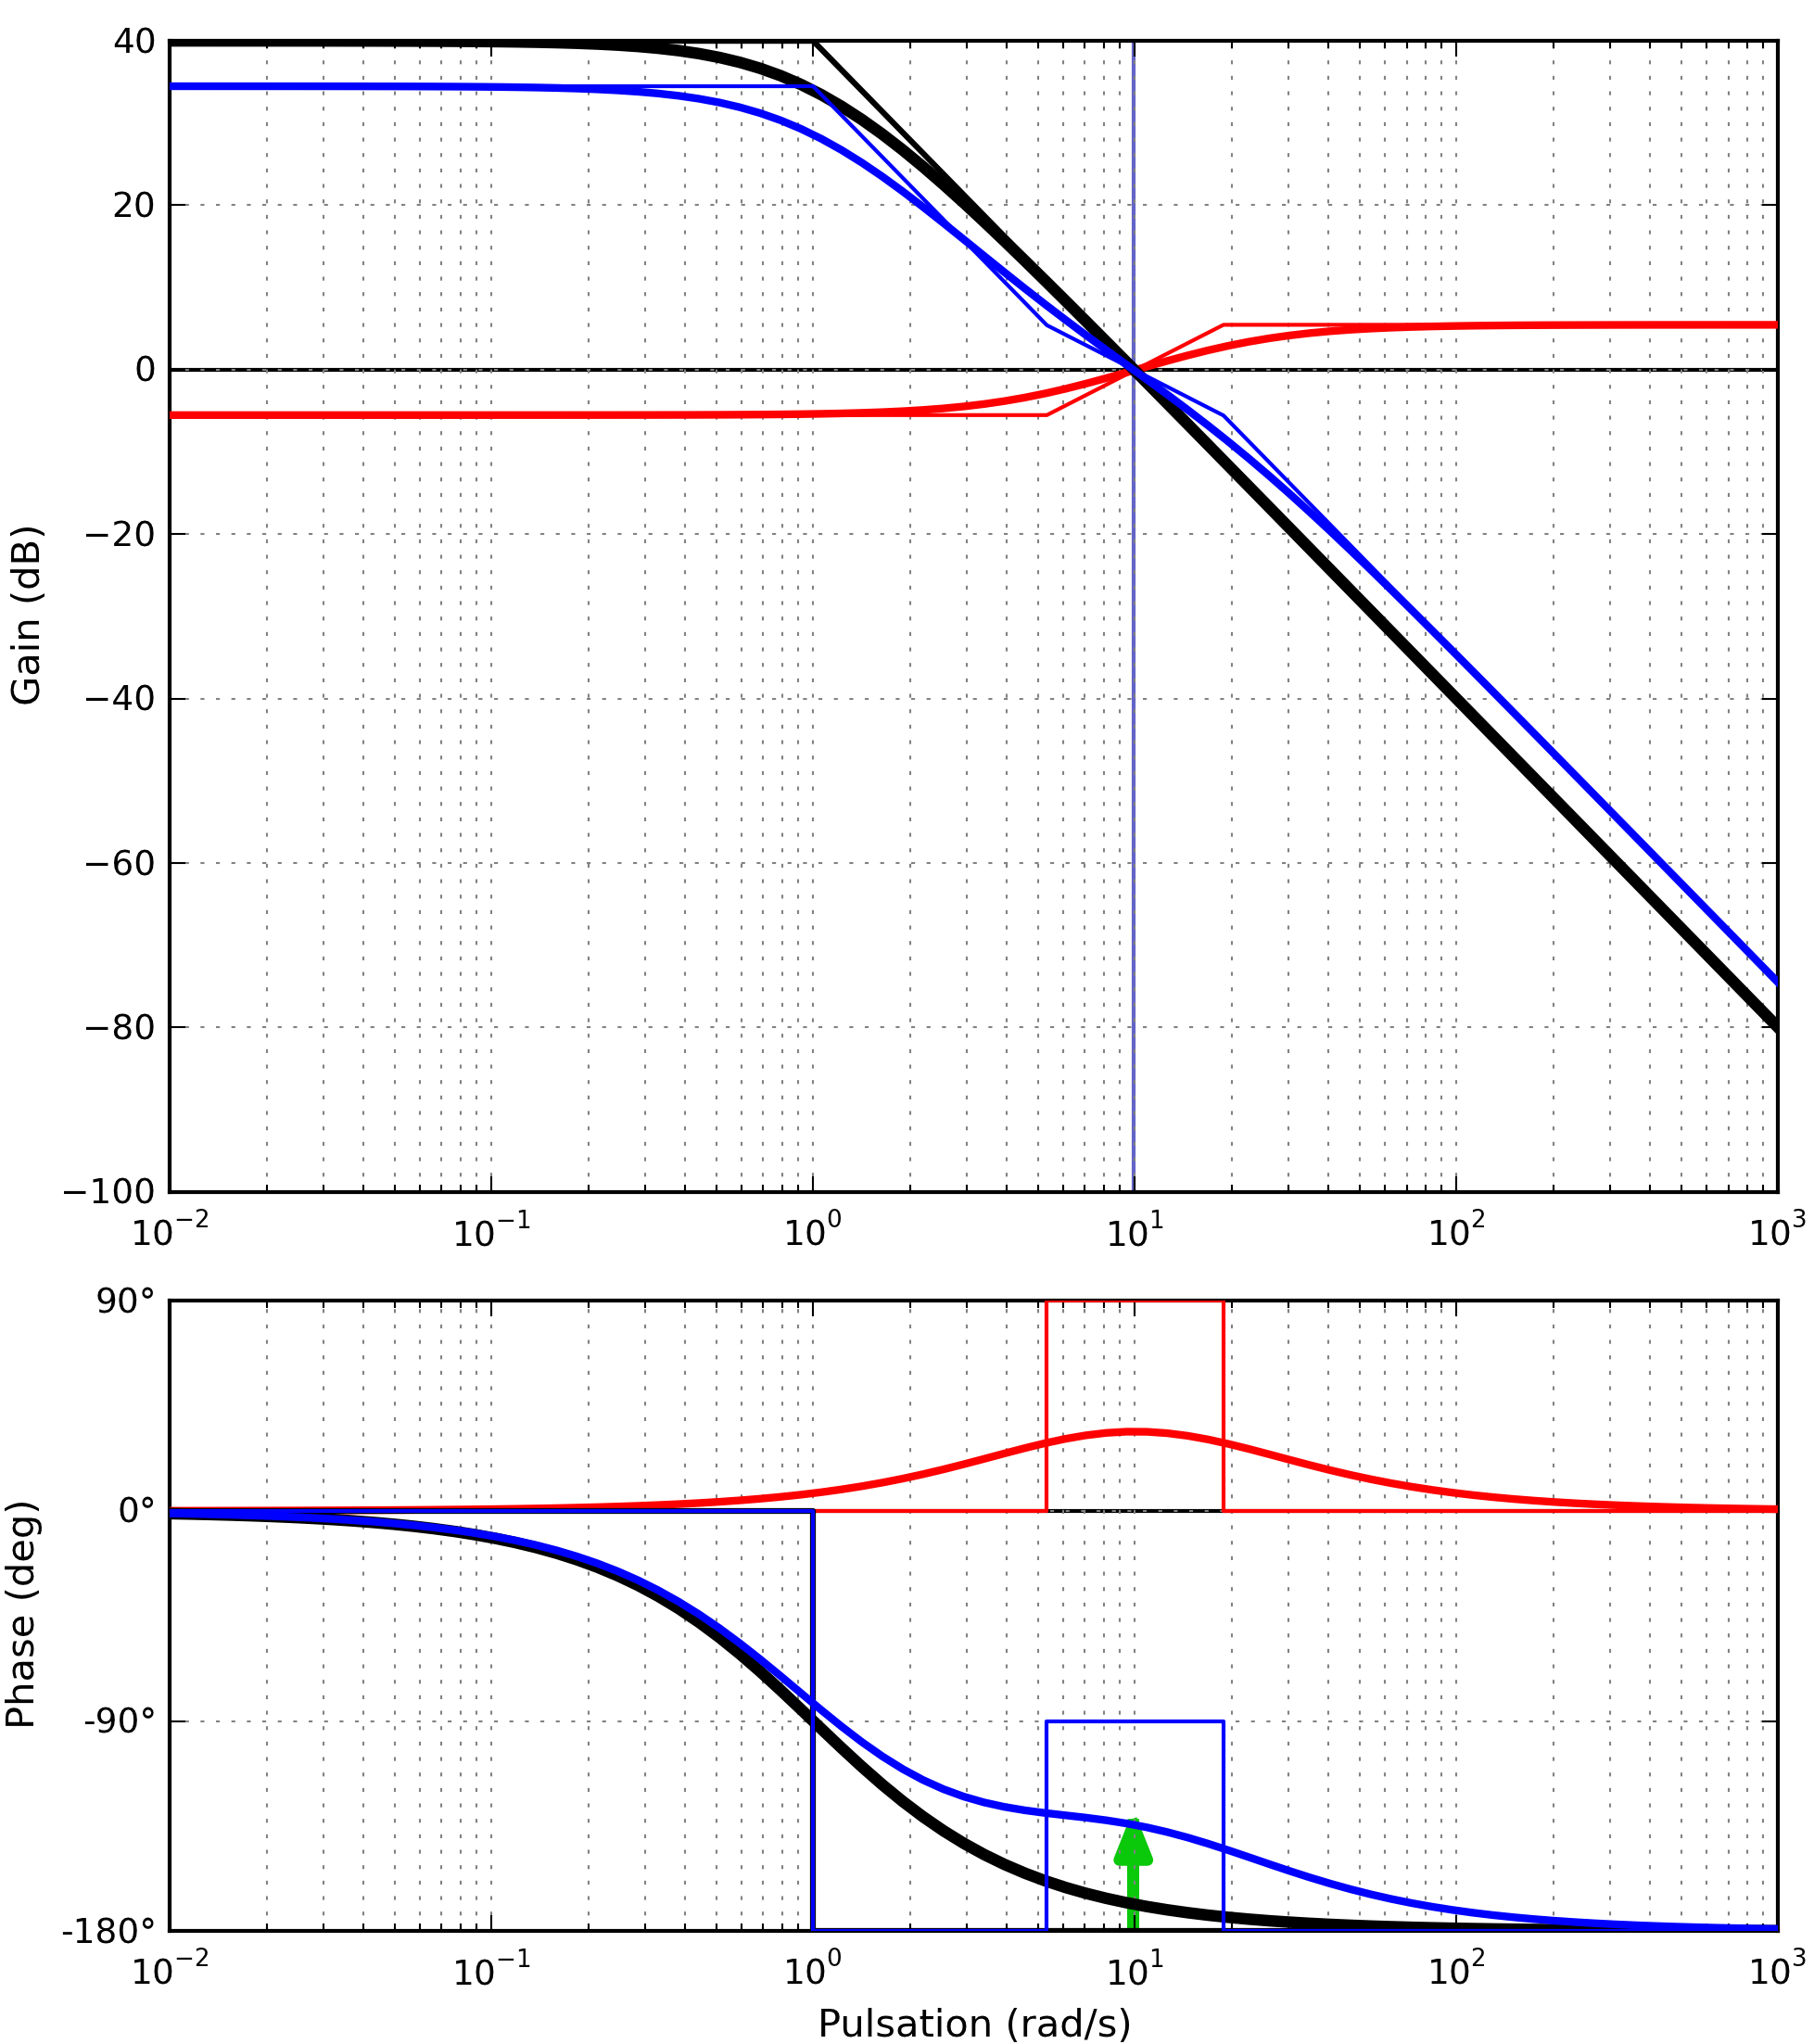
\includegraphics[width=.8\linewidth]{AP_BodeC.png}
%
%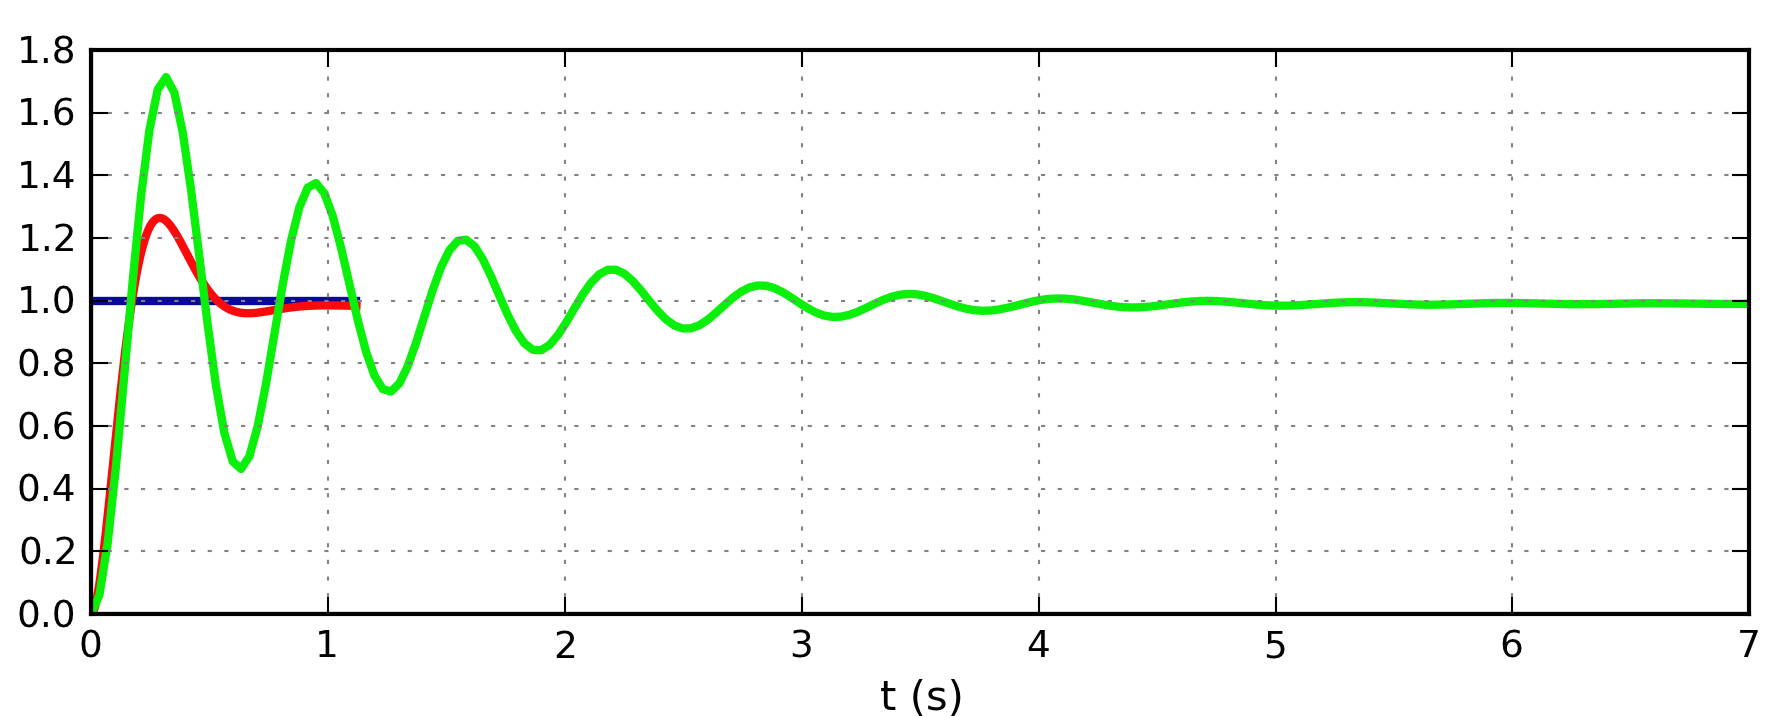
\includegraphics[width=.8\linewidth]{AP_corrige.png}
%\end{center}
%
%\fi
%
%\ifprof
%\else
%\begin{center}
%\rotatebox{90}{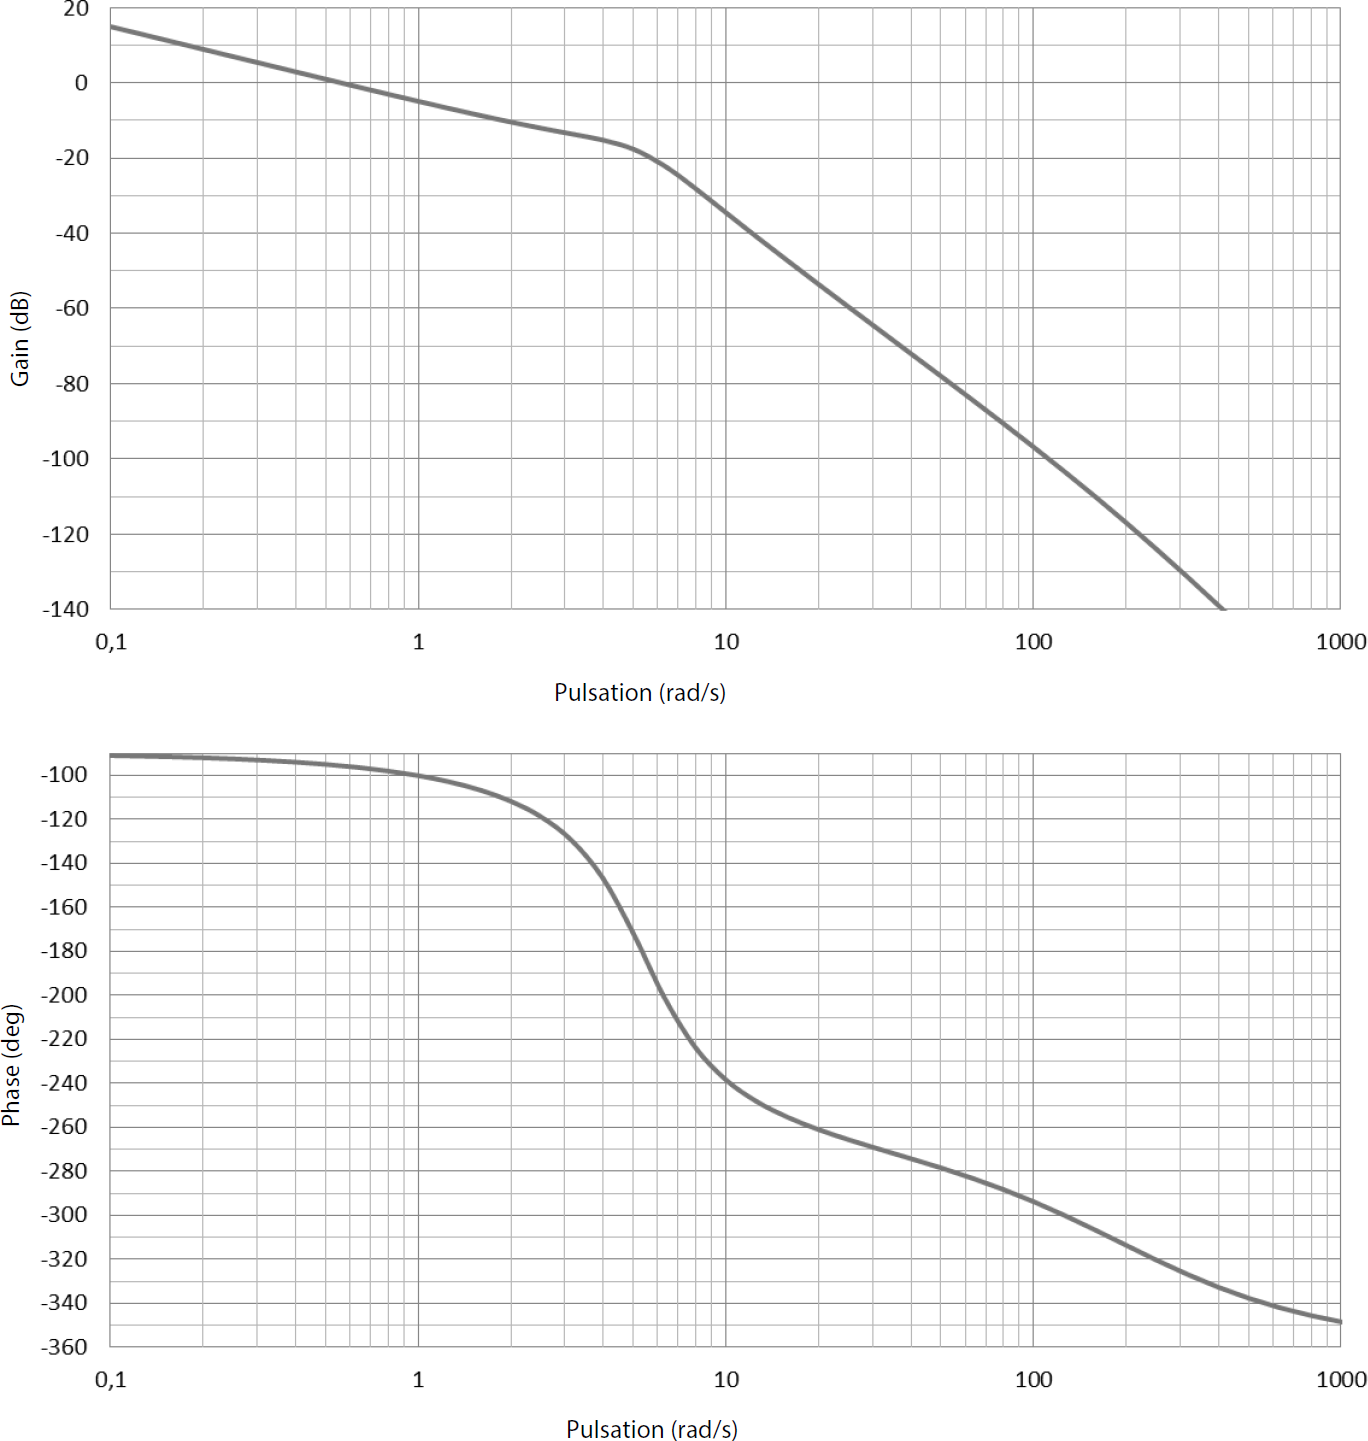
\includegraphics[width=.8\linewidth]{fig_04}}
%
%\rotatebox{90}{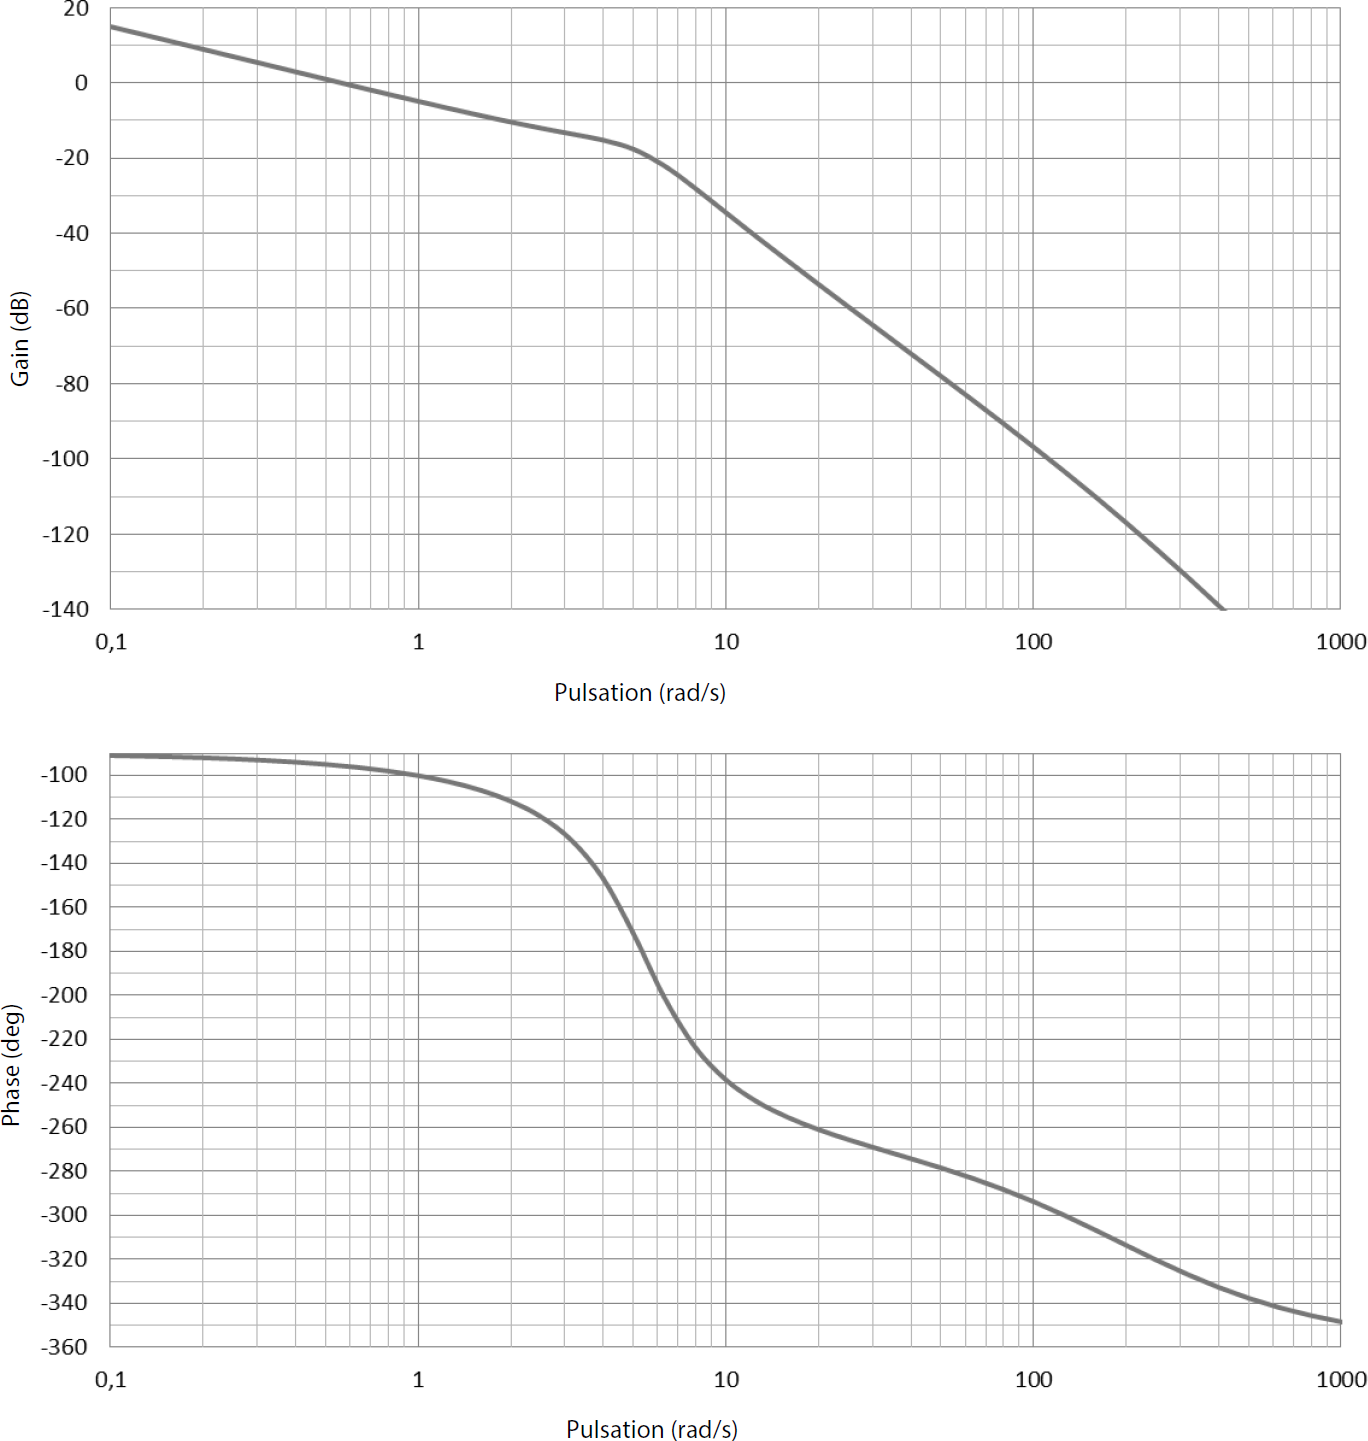
\includegraphics[width=.8\linewidth]{fig_04}}
%\end{center}
%
%\fi


%\end{document}